\documentclass[11pt,a4paper]{article}

\usepackage[spanish]{babel}
\usepackage[utf8]{inputenc}
\usepackage[T1]{fontenc}
\usepackage{geometry}
\usepackage{booktabs}
\usepackage{array}
\usepackage{graphicx}
\usepackage{xcolor}
\usepackage{hyperref}
\usepackage{enumitem}
\usepackage{tikz}
\usepackage{multirow}
\usepackage{colortbl}
\usepackage{placeins}
\usepackage{tabularx}
\usepackage{parskip}
\usepackage{longtable}
\usetikzlibrary{arrows.meta,babel,positioning,shapes.geometric,calc,patterns,shadows,fit}

\geometry{margin=2.2cm}
\hypersetup{colorlinks=true, linkcolor=black, urlcolor=blue!50!black}
\setlist[itemize]{noitemsep, topsep=3pt}
\setlist[enumerate]{noitemsep, topsep=3pt}
\newcommand{\code}[1]{\texttt{#1}}

\definecolor{offlinebg}{HTML}{E8F0FE}
\definecolor{onlinebg}{HTML}{FFF3E0}
\definecolor{storebg}{HTML}{F3E5F5}
\definecolor{offlineborder}{HTML}{1565C0}
\definecolor{onlineborder}{HTML}{E65100}
\definecolor{storeborder}{HTML}{7B1FA2}
\definecolor{barblue}{HTML}{1976D2}
\definecolor{bargreen}{HTML}{388E3C}
\definecolor{barorange}{HTML}{F57C00}
\definecolor{barred}{HTML}{D32F2F}
\definecolor{barteal}{HTML}{00897B}
\definecolor{tabheader}{HTML}{E3F2FD}

\begin{document}
\hypersetup{pageanchor=false}
\begin{titlepage}
\thispagestyle{empty}
\vspace*{1.7cm}
\begin{center}
  {\small\MakeUppercase{Proyecto final de Minería de Textos}}\\[2.2cm]
  {\bfseries\Huge WikiRAG-ES}\\[0.35cm]
  {\rule{0.62\textwidth}{0.6pt}}\\[0.85cm]
  {\Large Asistente RAG local sobre Wikipedia en español}\\[0.28cm]
  {\large Arquitectura agencial, recuperación híbrida y evaluación IR}\\[1.5cm]
  
\includegraphics[width=0.5\textwidth]{logo_wikirag.png}
\end{center}

\vfill
\noindent\rule{\textwidth}{0.4pt}\\[0.45cm]
\begin{minipage}[t]{0.46\textwidth}
  \small\MakeUppercase{Autores}\\[0.35cm]
  Lucas González Fiz\\[0.12cm]
  Adan González Rodríguez\\[0.12cm]
  Santiago Palomino Vazquez\\[0.12cm]
  Javier Pérez Robles
\end{minipage}\hfill
\vspace*{1.2cm}
\end{titlepage}
\hypersetup{pageanchor=true}
\tableofcontents
\newpage
\pagenumbering{arabic}

%% =========================================================================
\section{Resumen del Proyecto}
%% =========================================================================

Se ha diseñado e implementado un \textbf{asistente documental local} basado en la arquitectura de Recuperación Aumentada por Generación (\textit{Retrieval-Augmented Generation}, RAG). El sistema descarga, normaliza y procesa un corpus masivo real (Wikipedia en español), fragmentándolo en \textit{chunks} y generando representaciones vectoriales densas. A partir de estos datos, construye índices híbridos (FAISS y BM25) y ejecuta modelado de tópicos \textit{offline}, permitiendo a un Agente LLM enrutar y responder consultas complejas en lenguaje natural.

\begin{itemize}
  \item \textbf{Corpus:} 1\,000\,000 documentos de MIRACL-es (Wikipedia en español), con 200 consultas \textit{qrels} de evaluación.
  \item \textbf{Escala de indexación:} 1\,140\,063 \textit{chunks} procesados e indexados.
  \item \textbf{Motor LLM:} \code{gemma4:e4b} operando íntegramente en local a través de Ollama.
  \item \textbf{Recuperación:} Sistema híbrido que fusiona recuperación semántica (FAISS) y léxica (BM25) mediante \textit{Reciprocal Rank Fusion} (RRF), con \textit{reranking} opcional por \textit{cross-encoder}.
  \item \textbf{Eficiencia:} Carga parcial de índices por modo de evaluación, ruta rápida para herramientas deterministas y cuantización vectorial TurboVec que reduce la memoria utilizada por los vectores en un 93,4\,\%.
\end{itemize}

%% =========================================================================
\section{Requisitos técnicos}
%% =========================================================================

\subsection{Módulo para cada temática}

Esta es la lista de los requisitos técnicos del proyecto.

\begin{table}[htbp]
\centering
\small
\rowcolors{2}{tabheader!40}{white}
\begin{tabularx}{\textwidth}{l l X}
\toprule
\rowcolor{tabheader} \textbf{Requisito} & \textbf{Módulo} & \textbf{Descripción} \\
\midrule
Embeddings & \code{indexing/embeddings.py} & Modelo Sentence Transformers multilingüe (384-dim). \\
Modelado de tópicos & \code{topics/modeling.py} & Agrupación semántica \textit{offline} con BERTopic/NMF. \\
Resumen extractivo & \code{summarization/extractive.py} & TextRank sobre grafos + MMR para penalizar redundancia. \\
LLM Local & \code{llm/ollama.py} & Conexión nativa con Ollama, hiperparámetros ajustados. \\
Pipeline RAG & \code{retrieval/hybrid.py} & Fusión híbrida FAISS + BM25 mediante RRF, independiente de escalas de \textit{score}. \\
Router Agencial & \code{agents/router.py} & Enrutado híbrido: atajos deterministas por regex y desambiguación con el LLM (salida JSON). \\
\midrule
\textit{Innovación} & \code{indexing/turbovec\_store.py} & Compresión extrema de vectores mediante cuantización por anchura de bits (TurboQuant). \\
\bottomrule
\end{tabularx}
\caption{Mapeo de requisitos del enunciado y módulos desarrollados.}
\end{table}

\newpage
\subsection{Archivos entregados}

El proyecto se acompaña de los siguientes archivos:

\begin{table}[htbp]
\centering
\small
\rowcolors{2}{tabheader!40}{white}
\begin{tabularx}{\textwidth}{l X}
\toprule
\rowcolor{tabheader} \textbf{Ruta del archivo o directorio} & \textbf{Contenido y función} \\
\midrule
\code{src/wikirag\_es/} & Código fuente completo de la librería Python del paquete \code{wikirag-es}. \\
\code{data/processed/miracl\_es\_corpus\_1M.jsonl} & Corpus local de 1\,000\,000 documentos MIRACL-es. \\
\code{data/reports/miracl\_es\_eval.jsonl} & 200 consultas de evaluación con sus documentos relevantes disponibles dentro del subconjunto local. \\
\code{data/indexes/default/} & Índices FAISS (Flat) y BM25 generados sobre 1\,140\,063 fragmentos. \\
\code{data/reports/doc\_eval\_*.json} & Reportes de evaluación IR reproducidos para 50 consultas etiquetadas. \\
\code{data/reports/*bench*.json} & Resultados y métricas de los benchmarks empíricos de escalabilidad, latencia y compresión de memoria (HNSW, TurboVec). \\
\code{data/reports/miracl\_es\_corpus\_package.tar.gz} & Entregable comprimido del corpus local, consultas de evaluación y manifiesto. El informe de tópicos se entrega como \code{data/reports/topics.json}. \\
\bottomrule
\end{tabularx}
\caption{Estructura de entregables del sistema.}
\end{table}

\FloatBarrier

%% =========================================================================
\section{Entorno de Ejecución}
%% =========================================================================

\subsection{Tecnologías y librerías clave}

\begin{table}[htbp]
\centering
\small
\rowcolors{2}{tabheader!40}{white}
\begin{tabularx}{\textwidth}{l X}
\toprule
\rowcolor{tabheader} \textbf{Capa de software} & \textbf{Tecnología} \\
\midrule
Entorno y CLI & Python 3.12, Click; el entorno de auditoría actual tiene Click 8.3.0. \\
Modelado Vectorial & Sentence Transformers, modelo \code{paraphrase-multilingual-MiniLM-L12-v2}; el entorno de auditoría actual tiene Sentence Transformers 5.4.1 y PyTorch 2.11.0+cu128. \\
Bases de Datos Vectoriales & FAISS CPU (IndexFlatIP / IndexHNSWFlat) en el entorno de benchmark original; TurboVec como dependencia opcional para cuantización a 4 bits. \\
Recuperación Léxica y \textit{Reranking} & BM25Okapi (\code{rank-bm25}) y cross-encoder \code{mmarco-mMiniLMv2-L12} \\
Motor de Inferencia & Ollama (servidor local), modelo \code{gemma4:e4b} \\
Procesamiento Analítico & BERTopic (UMAP+HDBSCAN), NetworkX (PageRank/TextRank) \\
\bottomrule
\end{tabularx}
\caption{Stack tecnológico del proyecto.}
\end{table}

\subsection{Hardware utilizado en pruebas}

Para acelerar la generación de \textit{embeddings} de más de un millón de fragmentos se ha aprovechado aceleración por hardware (CUDA).

\begin{table}[htbp]
\centering
\rowcolors{2}{tabheader!40}{white}
\begin{tabularx}{\textwidth}{l X}
\toprule
\rowcolor{tabheader} \textbf{Componente} & \textbf{Especificación} \\
\midrule
Acelerador Gráfico (GPU) & NVIDIA GeForce RTX 5060 Ti (8\,GB VRAM) \\
Motor Vectorial & PyTorch con backend CUDA en la corrida de indexación; en la auditoría actual se detectó PyTorch 2.11.0+cu128, mientras que \code{faiss-cpu}, \code{bertopic} y \code{turbovec} no estaban instalados en el intérprete activo. \\
\bottomrule
\end{tabularx}
\caption{Especificaciones del servidor local utilizado en la corrida documentada.}
\end{table}

\FloatBarrier
\newpage
%% =========================================================================
\section{Arquitectura del Sistema}
%% =========================================================================

El flujo de trabajo se divide conceptualmente en dos grandes bloques: el procesamiento de datos por lotes (fase \textit{offline}) y la interacción con el LLM en tiempo real (fase \textit{online}).

\subsection{Diagrama de Flujo de Datos}

\begin{center}
\resizebox{0.9\linewidth}{!}{%
\begin{tikzpicture}[
  node distance=1.2cm and 1.6cm,
  module/.style={rectangle, rounded corners=6pt, draw=offlineborder!80, fill=offlinebg,
    align=center, minimum width=3.2cm, minimum height=1.2cm, font=\small\bfseries, drop shadow={opacity=0.2}},
  db/.style={cylinder, shape border rotate=90, aspect=0.25, draw=storeborder!80, fill=storebg,
    align=center, minimum width=2.8cm, minimum height=1.8cm, font=\small\bfseries, drop shadow={opacity=0.2}},
  agent/.style={rectangle, rounded corners=6pt, draw=onlineborder!80, fill=onlinebg,
    align=center, minimum width=3.2cm, minimum height=1.2cm, font=\small\bfseries, drop shadow={opacity=0.2}},
  arrow/.style={-{Latex[length=3mm]}, thick, draw=gray!80}
]

% Nodos FASE OFFLINE
\node[module] (corpus) {Corpus MIRACL-es\\(1M docs)};
\node[module, right=of corpus] (clean) {Limpieza y\\Normalización};
\node[module, right=of clean] (chunk) {Chunking\\(900 chars)};
\node[module, right=of chunk] (embed) {Encoder GPU\\(SentenceTrf)};

\node[db, below=1.5cm of embed] (vector) {FAISS + BM25\\(1,14M chunks)};
\node[db, below=1.5cm of clean] (topics) {Modelos Offline\\(BERTopic)};

% Enlaces FASE OFFLINE
\draw[arrow] (corpus) -- (clean);
\draw[arrow] (clean) -- (chunk);
\draw[arrow] (chunk) -- (embed);
\draw[arrow] (embed) -- (vector);
\draw[arrow] (clean) -- (topics);

% Nodos FASE ONLINE
\node[agent, below=2.5cm of vector] (router) {Agente Router};
\node[agent, left=of router] (llm) {LLM Local\\(Ollama)};
\node[module, draw=gray, fill=white, left=of llm] (user) {Usuario};
\node[module, draw=gray, fill=white, right=of router] (answer) {Respuesta\\Aumentada};

% Enlaces FASE ONLINE
\draw[arrow] (user) -- (llm);
\draw[arrow] (llm) -- (router);
\draw[arrow, dashed] (vector) -- node[right, font=\footnotesize]{RRF} (router);
\draw[arrow, dashed] (topics) -- (router);
\draw[arrow] (router) -- (answer);

% Agrupaciones con FIT
\node[draw=offlineborder, dotted, thick, inner sep=14pt, fit=(corpus) (embed) (topics) (vector)] (offlinebox) {};
\node[font=\footnotesize\bfseries, text=offlineborder, anchor=north west, inner sep=4pt] at (offlinebox.north west) {FASE OFFLINE (Indexación)};

\node[draw=onlineborder, dotted, thick, inner sep=14pt, fit=(user) (answer) (router)] (onlinebox) {};
\node[font=\footnotesize\bfseries, text=onlineborder, anchor=north west, inner sep=4pt] at (onlinebox.north west) {FASE ONLINE (Inferencia)};

\end{tikzpicture}
}
\end{center}

\subsection{Diseño Agencial del Router}

En lugar de construir un RAG tradicional donde toda pregunta activa incondicionalmente la base vectorial, se ha implementado un \textbf{Agente Router} de dos niveles. La clase \code{AssistantAgent} aplica primero atajos deterministas por expresiones regulares para disparadores explícitos (resumen, fecha, tópicos, peticiones web y consultas de actualidad) y, ante consultas ambiguas, delega la decisión en el \textbf{LLM}, que selecciona la herramienta devolviendo un objeto JSON (\code{function-calling} ligero). Si el LLM no está disponible o su salida es inválida, el sistema recae con seguridad en la herramienta RAG. Esto ahorra tokens, reduce la latencia previa a mostrar la herramienta activa y mantiene un comportamiento robusto. El agente conserva además \textbf{memoria conversacional}: solo reescribe las preguntas de seguimiento cuando hay referencias anafóricas reales al historial.

\begin{table}[htbp]
\centering
\small
\rowcolors{2}{tabheader!40}{white}
\begin{tabularx}{\textwidth}{l l X}
\toprule
\rowcolor{tabheader} \textbf{Herramienta} & \textbf{Patrón de activación} & \textbf{Ejecución algorítmica} \\
\midrule
\code{RagTool} & (Fallback por defecto) & Ejecuta FAISS y BM25, fusiona con RRF e inyecta fragmentos al LLM. \\
\code{SummaryTool} & \textit{resume, ideas principales...} & Calcula TextRank extractivo sobre el contexto recuperado y devuelve frases existentes. \\
\code{TopicTool} & \textit{tópicos/clusters del corpus...} & Extrae información del archivo JSON de clústeres de BERTopic. \\
\code{DateTool} & \textit{qué día es hoy...} & Devuelve la fecha actual formateada en español (día de la semana incluido). \\
\code{WebSearchTool} & \textit{internet, web, noticias, actualidad...} & Busca en DuckDuckGo información complementaria, la combina con contexto local y responde citando \code{[Web N]} cuando usa resultados externos. \\
\bottomrule
\end{tabularx}
\caption{Inventario de herramientas del Agente Router.}
\end{table}

Las respuestas generativas se emiten en \textit{streaming} mediante Ollama cuando pasan por el LLM. Las rutas deterministas sin LLM, como fecha y resumen extractivo, emiten texto por bloques o frases para que el usuario no espere a que termine toda la operación. Además, las fuentes mostradas al final de una respuesta RAG o web se filtran por citas explícitas: solo se listan aquellas que aparezcan realmente como \code{[Fuente N]} o \code{[Web N]} en la respuesta. Esto evita presentar como evidencias documentos recuperados por vecindad cuando el modelo ha declarado que no hay contexto suficiente.

\subsection{Resumen extractivo y determinismo}

El módulo de resumen no es un resumen abstractivo generado por el LLM. Es un \textbf{resumen extractivo}: selecciona frases literales presentes en el contexto recuperado o en el fichero de entrada. La implementación se encuentra en \code{summarization/extractive.py} y combina tres pasos:

\begin{enumerate}
  \item Segmentación del texto en frases suficientemente largas.
  \item Cálculo de embeddings por frase y construcción de un grafo de similitud coseno.
  \item Aplicación de TextRank/PageRank para centralidad y selección con MMR para penalizar redundancia.
\end{enumerate}

Cuando el usuario pregunta \textit{``Resume lo que tengas sobre X''}, el agente limpia la consulta para recuperar por el tema principal, obtiene contexto con RAG y después resume ese contexto. Antes de aplicar TextRank se eliminan cabeceras de contexto como \code{[Fuente N]}, \code{Ruta:} y \code{Texto:}; el resumen se calcula sobre el contenido documental, no sobre metadatos. Por tanto, el resumen es tan estable como lo sean la consulta efectiva y el contexto recuperado. Con el mismo índice, mismo \code{top\_k}, mismo historial conversacional y mismo contexto de entrada, el algoritmo extractivo debe devolver el mismo resultado. Si cambia el historial, se activa un índice aproximado, cambia el reranker o se recuperan fragmentos distintos, el resumen también puede cambiar.

La revisión del sistema detectó tres fuentes de variabilidad que debían controlarse: la intención explícita de resumen podía perderse si la reescritura conversacional eliminaba la palabra \textit{``resume''}; la consulta de resumen podía incluir verbos de instrucción que deterioraban el recuperador; y la selección MMR podía desempatar frases equivalentes sin orden estable. La corrección aplicada hace que los disparadores explícitos del usuario tengan prioridad sobre la reescritura, que la búsqueda se haga por el tema limpio y que los empates del resumen se resuelvan por orden de frase. Esto no convierte el RAG completo en determinista bajo cualquier configuración, pero sí hace determinista el resumen cuando recibe el mismo texto de entrada.

\FloatBarrier
\newpage
%% =========================================================================
\section{Corpus de Conocimiento (MIRACL-es)}
%% =========================================================================

Se eligió MIRACL (\textit{Multilingual Information Retrieval Across a Continuum of Languages}) como corpus principal por tres motivos fundamentales:
\begin{enumerate}
  \item Contiene volcados directos de Wikipedia, asegurando alta densidad informativa.
  \item Garantiza gramática y vocabulario nativo en español.
  \item Proporciona conjuntos de evaluación manual (\textit{qrels}) validados por expertos, indispensables para poder medir objetivamente el rendimiento del sistema RAG.
\end{enumerate}

\begin{table}[htbp]
\centering
\rowcolors{2}{tabheader!40}{white}
\begin{tabularx}{\textwidth}{l X}
\toprule
\rowcolor{tabheader} \textbf{Métrica del Corpus} & \textbf{Volumen final} \\
\midrule
Documentos indexados & 1\,000\,000 documentos MIRACL-es \\
\textit{Chunks} resultantes indexados & 1\,140\,063 fragmentos de texto \\
Consultas de evaluación (\textit{qrels} expertos) & 200 \\
Tamaño persistido (FAISS + \code{embeddings.npy}) & 3,50\,GB de vectores \\
Tópicos offline entregados & BERTopic sobre 100\,198 documentos, 1\,413 filas de \code{topic\_info} \\
\bottomrule
\end{tabularx}
\caption{Estadísticas del corpus de entrega tras la fase de ingestión.}
\end{table}

\subsection{Auditoría del modelado de tópicos}

El fichero \code{data/reports/topics.json} fue generado con BERTopic sobre 100\,198 documentos. Es importante distinguir entre \textit{clusters reales} y el identificador especial \code{-1}. En BERTopic, \code{-1} no representa un tema semántico útil, sino documentos considerados \textit{outliers} o no asignados a ningún cluster. Por tanto, el reporte actual no contiene siete tópicos: contiene \textbf{1\,412 clusters reales} más \textbf{34\,698 documentos outlier}.

\begin{table}[htbp]
\centering
\rowcolors{2}{tabheader!40}{white}
\begin{tabularx}{\textwidth}{X r}
\toprule
\rowcolor{tabheader} \textbf{Campo del reporte de tópicos} & \textbf{Valor} \\
\midrule
Método & BERTopic \\
Documentos modelados & 100\,198 \\
Filas en \code{topic\_info} & 1\,413 \\
Clusters reales, excluyendo \code{-1} & 1\,412 \\
Documentos outlier en \code{-1} & 34\,698 \\
\bottomrule
\end{tabularx}
\caption{Lectura correcta del reporte \code{topics.json}.}
\end{table}

La confusión aparece cuando la herramienta de tópicos muestra solo los primeros resultados por brevedad: si se limita la salida a unas pocas filas y una de ellas es \code{-1}, puede parecer que el corpus tiene únicamente unos pocos tópicos útiles. La lectura correcta es que la lista presentada en chat es una \textbf{vista resumida} de los clusters mayores, no el número total de clusters generados.

\begin{center}
\small
\rowcolors{2}{tabheader!40}{white}
\begin{longtable}{r r p{0.68\textwidth}}
\caption{Veinticinco clusters reales más grandes del reporte BERTopic, excluyendo \code{-1}. El listado completo está en \code{data/reports/topics.json}.}\\
\toprule
\rowcolor{tabheader} \textbf{Cluster} & \textbf{Docs} & \textbf{Representación principal} \\
\midrule
\endfirsthead
\toprule
\rowcolor{tabheader} \textbf{Cluster} & \textbf{Docs} & \textbf{Representación principal} \\
\midrule
\endhead
0 & 757 & poesía, modernismo, ramón, literatura, revista, poeta \\
1 & 660 & educación, universidad, escuelas, universidades, secundaria, alumnos \\
2 & 559 & transporte, carreteras, autobuses, tren, líneas, estación \\
3 & 499 & cocina, gastronomía, platos, arroz, carne, queso \\
4 & 498 & mesoamérica, tlaxcala, pueblos, mayas, maya, teotihuacán \\
5 & 453 & clima, temperaturas, precipitaciones, mm, lluvias, temperatura \\
6 & 440 & canadá, ontario, brunswick, manitoba, nuevo brunswick, alberta \\
7 & 361 & televisión, hd, alta definición, radio, televisión alta, canal \\
8 & 293 & mozart, bach, schubert, johann, wolfgang, johann sebastian \\
9 & 277 & unidades, kilogramo, unidad, litro, sistema internacional, metro \\
10 & 262 & carter, bush, clinton, reagan, jimmy carter, jimmy \\
11 & 236 & franco, francisco franco, azaña, francisco, batalla, civil española \\
12 & 235 & cine, cine mexicano, mexicano, buñuel, película, películas \\
13 & 231 & alfonso, aragón, castilla, fernando, sancho, alfonso vi \\
14 & 230 & primer ministro, ministros, asamblea, ministro, parlamento, cámara \\
15 & 226 & corán, islam, mahoma, musulmanes, profeta, árabe \\
16 & 225 & religión, iglesia, católicos, católica, protestantes, religiones \\
17 & 220 & río, ríos, cuenca, afluentes, aguas, lago \\
18 & 213 & fármaco, medicamento, farmacia, farmacéutico, fármacos, medicamentos \\
19 & 212 & bolívar, simón, simón bolívar, bolivia, caracas, sucre \\
20 & 202 & cerebelo, nervioso, sistema nervioso, fibras, cerebro, encéfalo \\
21 & 200 & vino, vinos, cerveza, uva, moscatel, uvas \\
22 & 200 & presidente, presidente chile, nación argentina, presidente nación, chile, constitución \\
23 & 199 & magnético, campo magnético, maxwell, campo, ecuaciones maxwell, ecuaciones \\
24 & 199 & karate, taekwondo, ryu, marciales, marcial, artes marciales \\
\bottomrule
\end{longtable}
\end{center}

\FloatBarrier

%% =========================================================================
\section{Resultados de Evaluación IR}
%% =========================================================================

El rendimiento de recuperación se evaluó sobre una muestra de \textbf{50 consultas} de MIRACL-es (\textit{dev}) con $k=10$, comparando tres configuraciones del motor frente al mismo \textit{ground-truth}.

El conjunto de evaluación local no es el MIRACL completo: durante la adquisición se conservan las consultas cuyos documentos relevantes están disponibles dentro del subconjunto local de 1M documentos. Esto hace que las métricas sean válidas para comparar configuraciones internas del proyecto, pero no deben presentarse como el resultado oficial de MIRACL-es completo. Además, los reportes JSON guardan las listas recuperadas tal como salen del motor; pueden aparecer identificadores repetidos si dos estrategias recuperan el mismo documento. Las métricas se calculan sobre IDs únicos mediante \code{evaluate\_ids}, evitando contar dos veces el mismo documento relevante.

\subsection{Métricas obtenidas}

\begin{table}[htbp]
\centering
\rowcolors{2}{tabheader!40}{white}
\begin{tabularx}{\textwidth}{X c c c c}
\toprule
\rowcolor{tabheader} \textbf{Motor de Recuperación} & \textbf{P@10} & \textbf{R@10} & \textbf{MRR} & \textbf{nDCG@10} \\
\midrule
Motor Léxico (BM25) & 0,072 & 0,341 & 0,264 & 0,248 \\
Motor Semántico (FAISS) & 0,112 & 0,451 & 0,451 & 0,379 \\
\rowcolor{green!8} \textbf{Fusión Híbrida (FAISS+BM25, RRF)} & \textbf{0,108} & \textbf{0,482} & \textbf{0,542} & \textbf{0,435} \\
\bottomrule
\end{tabularx}
\caption{Métricas sobre el corpus 1M de entrega (50 \textit{queries}, $k=10$).}
\end{table}

\subsection{Qué mide cada métrica}

El proyecto mide la recuperación antes de la generación del LLM. Esto es deliberado: en un sistema RAG, si el recuperador no coloca evidencia correcta en las primeras posiciones, el generador no puede responder de forma fiable aunque el modelo sea bueno.

\begin{table}[htbp]
\centering
\small
\rowcolors{2}{tabheader!40}{white}
\begin{tabularx}{\textwidth}{l X X}
\toprule
\rowcolor{tabheader} \textbf{Métrica} & \textbf{Definición} & \textbf{Interpretación para RAG} \\
\midrule
\textit{Precision@k} & Proporción de resultados del top-$k$ que son relevantes. & Mide ruido en el contexto. Puede ser baja si los qrels tienen pocos relevantes por consulta. \\
\textit{Recall@k} & Proporción de documentos relevantes esperados que aparecen en el top-$k$. & Mide cobertura; es clave para saber si el contexto contiene evidencia suficiente. \\
\textit{MRR} & Recíproco de la posición del primer resultado relevante. & Mide si la primera evidencia útil aparece arriba, donde más influye en el prompt. \\
\textit{nDCG@k} & Ganancia descontada normalizada por posición. & Mide calidad global del ranking, premiando relevantes en posiciones tempranas. \\
\textit{Latencia} & Tiempo medio por consulta o por búsqueda semántica aislada. & Mide viabilidad interactiva, pero depende mucho de si se incluye BM25, FAISS, LLM o solo el índice vectorial. \\
\textit{Memoria vectorial} & Tamaño ocupado por índices y embeddings. & Permite comparar FAISS \textit{float32} frente a cuantización TurboVec. \\
\bottomrule
\end{tabularx}
\caption{Métricas implementadas y usadas en los reportes de evaluación.}
\end{table}

Además de estas métricas, el sistema podría extenderse con métricas de generación final: ROUGE o BERTScore para resumen si existieran referencias humanas, precisión de citas para comprobar si cada afirmación está soportada, \textit{faithfulness/groundedness} para medir alucinaciones, Exact Match/F1 para preguntas cerradas, latencia \textit{end-to-end} del chat y tasa de \textit{fallback} del router. No se reportan como métricas principales porque la entrega cuenta con qrels expertos de recuperación, no con respuestas humanas completas ni resúmenes de referencia.

\subsection{Análisis: del baseline al sistema completo}

La progresión por capas evidencia el aporte de cada componente sobre el \textit{baseline} léxico:

\begin{itemize}
  \item \textbf{Híbrido vs. baselines:} la \textit{Reciprocal Rank Fusion} (RRF) mejora consistentemente el \textit{Recall@10}, el MRR y el nDCG@10 respecto a BM25 y FAISS por separado. El léxico aporta coincidencias exactas y el semántico captura paráfrasis. Su fusión eleva el MRR a \textbf{0,542} y el nDCG@10 a \textbf{0,435}, demostrando que no solo se recuperan más documentos relevantes, sino que se posicionan de forma mucho más óptima en el ranking.
  \item \textbf{Coste de escala:} BM25 sobre 1\,140\,063 fragmentos es el cuello de botella de la evaluación. Por ello se implementó carga parcial de índices: el modo léxico no carga FAISS ni el modelo de embeddings, y los benchmarks no cargan textos de fragmentos cuando solo necesitan \code{doc\_id}.
  \item \textbf{Lectura del MRR (0,542):} en la muestra documentada, el primer documento relevante aparece de media alrededor de la segunda posición. Es una métrica central para RAG porque el LLM atiende preferentemente a las primeras fuentes del \textit{prompt}.
  \item \textbf{Precisión y \textit{qrels}:} \textit{Precision@10} se mantiene moderada porque MIRACL-es marca pocos documentos relevantes por consulta. Recuperar 10 implica un techo de precisión bajo por construcción, de modo que \textit{Recall@10} y MRR son indicadores más informativos.
  \item \textbf{Impacto del Reranking (Cross-Encoder):} En una evaluación separada sobre 200 consultas y el índice HNSW, la activación de la etapa de \textit{reranking} logra una mejora sustancial adicional. El MRR asciende de 0,481 a \textbf{0,636} y el \textit{Recall@10} pasa de 0,540 a \textbf{0,640}. Esta comparación no debe mezclarse directamente con la tabla de 50 consultas, pero sí muestra que el \textit{cross-encoder} reordena eficazmente los candidatos de la fase híbrida.
\end{itemize}

\FloatBarrier
\newpage

%% =========================================================================
\section{Escalabilidad RAG según el Tamaño del Corpus}
%% =========================================================================

Para justificar el uso de Big Data en arquitecturas RAG, se ha diseñado un benchmark de escalabilidad que evalúa cómo se comporta la calidad y el rendimiento del sistema híbrido al variar el volumen de fragmentos indexados. Se evaluaron colecciones de $100\,000$, $500\,000$ y la totalidad de $1\,140\,063$ \textit{chunks}.

\begin{table}[htbp]
\centering
\rowcolors{2}{tabheader!40}{white}
\begin{tabularx}{\textwidth}{X c c c c}
\toprule
\rowcolor{tabheader} \textbf{Tamaño del Corpus (chunks)} & \textbf{P@10} & \textbf{R@10} & \textbf{MRR} & \textbf{Latencia Media} \\
\midrule
100\,000 & 0,045 & 0,146 & 0,157 & 313 ms \\
500\,000 & 0,085 & 0,370 & 0,373 & 1546 ms \\
1\,140\,063 & 0,109 & 0,482 & 0,542 & 3520 ms \\
\bottomrule
\end{tabularx}
\caption{Evolución del desempeño en función de la cantidad de documentos procesados. (Recuperador Híbrido, 50 queries, k=10)}
\end{table}

\begin{figure}[htbp]
    \centering
    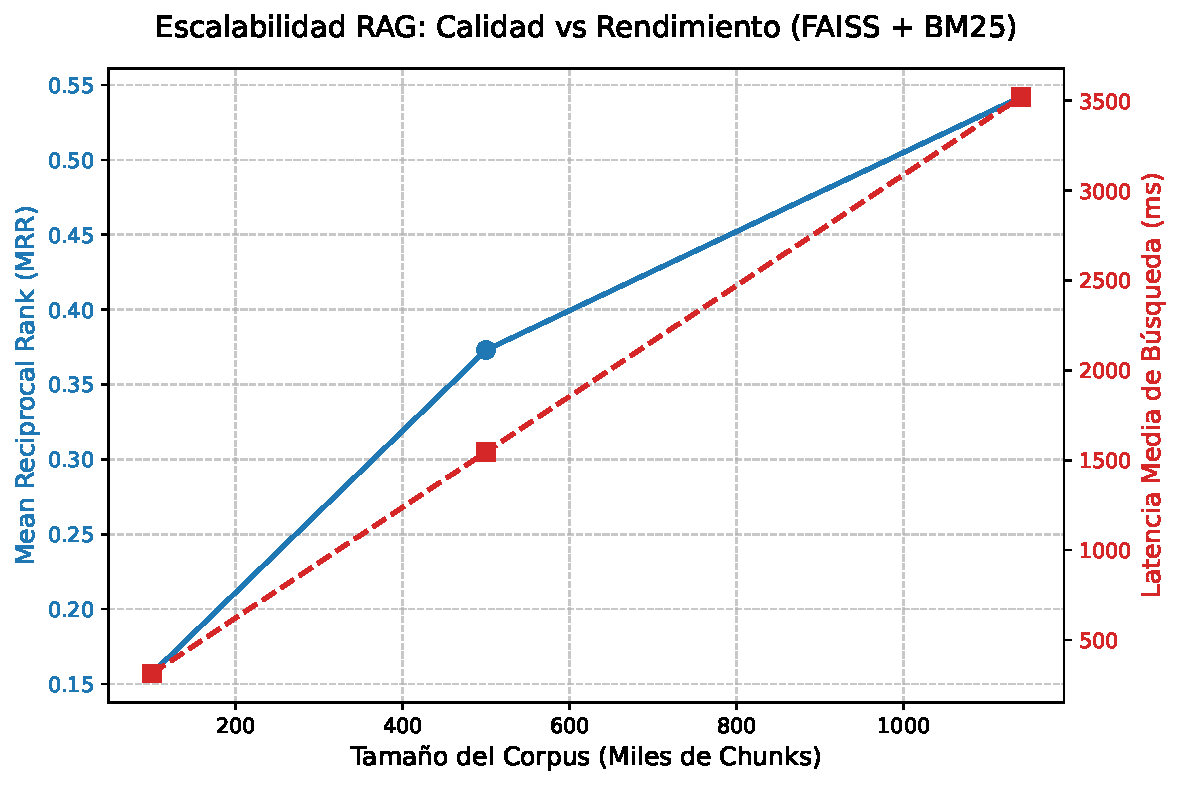
\includegraphics[width=0.85\textwidth]{scaling_plot.pdf}
    \caption{Relación entre calidad de recuperación (MRR) y degradación del rendimiento (latencia) al incrementar el tamaño del corpus.}
\end{figure}

\textbf{Análisis de los resultados:}
\begin{enumerate}
    \item \textbf{Mejora de la calidad de recuperación:} Se observa empíricamente que, a medida que el modelo dispone de más texto fuente, la probabilidad de recuperar el fragmento correcto aumenta. Escalar de 100k a 1.1M \textit{chunks} eleva el MRR de 0,157 a 0,542 y mejora significativamente el \textit{Recall}.
    \item \textbf{Impacto en el rendimiento:} Como era de esperar, la latencia total de la recuperación crece de forma aproximadamente lineal con el número de \textit{chunks}, alcanzando 3.520 ms por consulta al procesar 1\,140\,063 fragmentos. Cabe destacar que el principal cuello de botella de esta métrica proviene del motor léxico BM25, ejecutado en Python puro, mientras que la parte semántica vectorial puede optimizarse fuertemente.
    \item \textbf{Justificación arquitectónica:} Este aumento en la latencia y en el consumo de memoria al evaluar grandes volúmenes de documentos justifica la integración de las optimizaciones descritas en las siguientes secciones: la \textbf{Indexación HNSW} (para reducir el tiempo de búsqueda semántica en FAISS) y la cuantización \textbf{TurboVec} (para optimizar el uso de memoria RAM).
\end{enumerate}

%% =========================================================================
\section{Indexación Aproximada (HNSW)}
%% =========================================================================

La búsqueda semántica exacta (\code{IndexFlatIP}) recorre 1\,140\,063 vectores en cada consulta, con coste lineal $O(N)$. Para reducir esa latencia se implementó una variante aproximada con \textbf{HNSW} (\textit{Hierarchical Navigable Small World}), activable mediante \code{--index-type hnsw}.

HNSW representa los embeddings como un grafo navegable. En vez de comparar la consulta con todos los vectores, explora vecinos prometedores y converge rápidamente hacia zonas relevantes del espacio semántico. En FAISS se configuró con \code{IndexHNSWFlat}, \code{M=32}, \code{efConstruction=200} y \code{efSearch=64}, priorizando una búsqueda rápida sin modificar los embeddings originales.

\begin{table}[htbp]
\centering
\rowcolors{2}{tabheader!40}{white}
\begin{tabularx}{\textwidth}{X c c c}
\toprule
\rowcolor{tabheader} \textbf{Tamaño del índice} & \textbf{FAISS Flat} & \textbf{FAISS HNSW} & \textbf{Reducción} \\
\midrule
100\,000 vectores & 5,156 ms & 0,165 ms & 31,2x \\
500\,000 vectores & 25,720 ms & 0,415 ms & 62,0x \\
1\,140\,063 vectores & 59,579 ms & 0,434 ms & 137,3x \\
\bottomrule
\end{tabularx}
\caption{Comparativa corregida de latencia semántica exacta frente a HNSW. Se mide la mediana de ms/consulta con ejecución query-a-query, 200 consultas, $k=10$, 5 repeticiones, 1 warmup y 1 hilo FAISS.}
\end{table}

\textit{Corrección metodológica:} la tabla anterior del informe usaba una única búsqueda batched de FAISS y daba un resultado no defendible: HNSW aparecía con menos latencia en 1,14M que en 500k vectores. Se ha regenerado el benchmark midiendo cada consulta por separado, igualando la metodología entre índices, fijando un hilo de FAISS y tomando la mediana de cinco repeticiones. Con esta medición, Flat crece de forma clara con el tamaño del índice y HNSW también aumenta de 100k a 500k, quedando prácticamente estabilizado entre 500k y 1,14M por el carácter sublineal de la navegación en grafo.

\begin{center}
\begin{tikzpicture}
  \node[anchor=east, font=\small\bfseries] at (-0.2, 1.6) {FAISS Flat};
  \node[anchor=east, font=\small\bfseries] at (-0.2, 0.5) {FAISS HNSW};

  \fill[barred, rounded corners=2pt, drop shadow={opacity=0.3}] (0, 1.2) rectangle (10, 2.0);
  \node[white, font=\small\bfseries] at (5, 1.6) {59,6 ms};

  \fill[bargreen, rounded corners=2pt, drop shadow={opacity=0.3}] (0, 0.1) rectangle (0.07, 0.9);
  \node[right, font=\small\bfseries, bargreen] at (0.17, 0.5) {0,434 ms};

  \draw[-{Latex}, thin, gray] (0,-0.2) -- (10.5,-0.2);
  \foreach \x/\l in {0/0, 2.5/15, 5/30, 7.5/45, 10/60} {
    \draw[gray] (\x,-0.25) -- (\x,-0.15);
    \node[below, font=\tiny, gray] at (\x,-0.25) {\l\,ms};
  }
\end{tikzpicture}
\end{center}

HNSW es útil cuando el cuello de botella principal es el tiempo de respuesta. El resultado corregido muestra que \code{IndexFlatIP} crece con el tamaño del índice porque escanea todos los vectores, mientras que HNSW explora un grafo aproximado y se mantiene en órdenes de magnitud inferiores. La contrapartida es que la búsqueda deja de ser exacta, por lo que \code{IndexFlatIP} se mantiene como referencia reproducible y HNSW como opción de escalado.

\FloatBarrier
\newpage

%% =========================================================================
\section{Benchmark de Cuantización (TurboVec)}
%% =========================================================================

Escalar a millones de documentos presenta una barrera física: los vectores \textit{float32} colapsan la memoria RAM. Para solucionarlo, se implementó un motor secundario \textbf{TurboVec}, que cuantiza cada componente de los vectores a 4 bits (esquema TurboQuant de anchura de bits sobre un \textit{IdMapIndex}).

\begin{table}[htbp]
\centering
\rowcolors{2}{tabheader!40}{white}
\begin{tabularx}{\textwidth}{X c c c c}
\toprule
\rowcolor{tabheader} \textbf{Tipo de Índice vectorial} & \textbf{P@10} & \textbf{R@10} & \textbf{MRR} & \textbf{Memoria utilizada} \\
\midrule
Índice FAISS crudo (\textit{float32}) & 0,113 & 0,451 & 0,451 & 3,50\,GB \\
Índice TurboVec Cuantizado (4-bit) & 0,111 & 0,447 & 0,456 & 232,6\,MB \\
\midrule
\multicolumn{4}{l}{\textit{Mejora de uso de memoria}} & \textbf{--93,4\,\%} \\
\bottomrule
\end{tabularx}
\caption{Comparativa de recursos semánticos (50 \textit{queries}, $k=10$). En la ejecución documentada, TurboVec redujo memoria de forma drástica. FAISS mantuvo menor latencia media en este benchmark de búsqueda persistida (54,0 vs. 77,3\,ms/consulta).}
\end{table}

\begin{center}
\begin{tikzpicture}
  \node[anchor=east, font=\small\bfseries] at (-0.2, 1.6) {FAISS};
  \node[anchor=east, font=\small\bfseries] at (-0.2, 0.5) {TurboVec};

  \fill[barred, rounded corners=2pt, drop shadow={opacity=0.3}] (0, 1.2) rectangle (10, 2.0);
  \node[white, font=\small\bfseries] at (5, 1.6) {3,50 GB};

  \fill[barteal, rounded corners=2pt, drop shadow={opacity=0.3}] (0, 0.1) rectangle (0.66, 0.9);
  \node[right, font=\small\bfseries, barteal] at (0.76, 0.5) {232,6 MB};

  \draw[-{Latex}, thin, gray] (0,-0.2) -- (10.5,-0.2);
  \foreach \x/\l in {0/0, 2.5/0.9, 5/1.75, 7.5/2.6, 10/3.5} {
    \draw[gray] (\x,-0.25) -- (\x,-0.15);
    \node[below, font=\tiny, gray] at (\x,-0.25) {\l\,GB};
  }
\end{tikzpicture}
\end{center}

TurboVec retiene el desempeño semántico casi a la perfección (caída de \textit{Recall@10} inferior a medio punto) y reduce la memoria utilizada por los vectores de 3,50\,GB a 232,6\,MB ($-$93,4\,\%). Extrapolado a colecciones mayores, este factor de compresión es clave para desplegar el asistente en ordenadores convencionales.

\FloatBarrier

\section{Comparativa de Técnicas Semánticas}

Una vez explicadas las dos optimizaciones principales, se separan dos preguntas distintas. La primera es de \textbf{latencia}: FAISS Flat frente a FAISS HNSW en búsqueda semántica pura. La segunda es de \textbf{memoria}: FAISS \textit{float32} frente a TurboVec cuantizado. Mezclar ambas en una única gráfica puede llevar a conclusiones confusas, porque TurboVec se evalúa principalmente por compresión y HNSW por tiempo de búsqueda.

La comparativa muestra dos estrategias complementarias:
\begin{itemize}
    \item \textbf{FAISS HNSW:} reduce de forma extrema la latencia de búsqueda al sustituir el escaneo exhaustivo por navegación aproximada en un grafo. En el benchmark corregido pasa de 59,579 ms a 0,434 ms por consulta sobre 1,14M vectores.
    \item \textbf{TurboVec Cuantizado (4 bits):} reduce de forma drástica la memoria persistida de los vectores y mantiene una calidad semántica muy parecida a FAISS exacto. Es la opción más adecuada cuando la limitación principal es almacenamiento o RAM, no necesariamente latencia.
\end{itemize}

FAISS exacto queda como referencia de calidad y reproducibilidad, HNSW como alternativa de baja latencia y TurboVec como alternativa de baja memoria. Según el escenario de despliegue, estas técnicas pueden elegirse de forma independiente o combinarse con la recuperación léxica BM25 y la fusión RRF del sistema híbrido.

\FloatBarrier
\newpage

%% =========================================================================
\section{Ejemplos Reales del Asistente RAG}
%% =========================================================================

Las siguientes interacciones fueron generadas desde la interfaz CLI interactiva del proyecto (\code{wikirag chat}).

% ------- Ejemplo 1 -------
\subsection{Consulta Factual (QREL Experto)}

\textbf{Usuario:} \textit{¿Cómo se convirtió Egipto en musulmán?} (consulta \textit{QREL} oficial del \textit{dev} de MIRACL-es).

\begin{quote}
Tras la muerte de Mahoma en el año 632 comenzó la expansión musulmana y, en un lapso de cien años, los árabes ocuparon Egipto [Fuente 5]. Durante los primeros 300 años el islam fue ganando adeptos hasta convertirse en la religión predominante de la sociedad egipcia [Fuente 1]\ldots
\end{quote}

\textit{La respuesta es trazable y recupera fragmentos relacionados con el artículo \code{es/33218}. En los reportes IR, sin embargo, los qrels exactos para esta consulta son \code{1452\#22} y \code{33218\#10}; por tanto, este ejemplo ilustra una respuesta cualitativamente coherente, pero no debe presentarse como acierto exacto del ground-truth en la evaluación automática.}
\vspace{0.3cm}
\textbf{Usuario:} \textit{¿Qué país formó la primera Infantería de Marina?}

\begin{quote}
La primera Infantería de Marina fue creada por Carlos I el 27 de febrero de 1537 al asignar de forma permanente a las escuadras de galeras del Mediterráneo las ``compañías viejas del mar de Nápoles'' [Fuente 1].
\end{quote}

\textit{El modelo responde con precisión histórica basándose en \code{es/63108\#3}. El conjunto de consultas y qrels queda en \code{data/reports/miracl\_es\_eval.jsonl}; los resultados agregados de evaluación se almacenan en \code{data/reports/doc\_eval\_*.json} y \code{eval\_hnsw\_hybrid*.json}.}

\newpage

% ------- Ejemplo 2 -------
\subsection{Rechazo Informado (Prevención de Alucinaciones)}

\textbf{Usuario:} \textit{¿Cuál es el horario de apertura del Museo del Prado?}

\begin{quote}
No se puede determinar el horario de apertura del Museo del Prado a partir del contexto proporcionado. Las fuentes ofrecen información sobre la ubicación, historia y obras del museo, pero no incluyen datos sobre sus horarios [Fuente 1, 3, 7].
\end{quote}

\textit{Se demuestra cómo el prompt conservador (\textit{"No inventes datos"}) reduce el riesgo de alucinación si los documentos recuperados de la Wikipedia no contienen horarios. Si la respuesta no contiene citas explícitas \code{[Fuente N]}, el sistema no muestra fuentes recuperadas solo por similitud.}

\vspace{0.3cm}
\textbf{Usuario:} \textit{¿Cuáles son los hiperparámetros de LangChain usados en el proyecto?}

\begin{quote}
El contexto proporcionado no contiene información sobre los hiperparámetros utilizados en el proyecto LangChain. Solo describe términos y conceptos relacionados con otros campos, por lo que no es posible responder con evidencia suficiente.
\end{quote}

\textit{El sistema rechaza responder con firmeza. Al buscar sobre LangChain en Wikipedia recupera conceptos técnicos aleatorios, pero al no encontrar la respuesta exacta, el LLM declara explícitamente su ignorancia. Este comportamiento conservador es deseable en un RAG, aunque no constituye una garantía formal de cero alucinaciones.}

% ------- Ejemplo 3 -------
\subsection{Llamada Agencial (Tool Routing)}

\textbf{Usuario:} \textit{¿Qué día es hoy?}

\begin{quote}
Hoy es \textit{[fecha calculada en ejecución]}.
\end{quote}

\textit{El agente no invoca a FAISS ni BM25, ya que deduce que la Wikipedia no contiene la respuesta al día actual, ejecutando el módulo \code{DateTool} internamente.}

\vspace{0.3cm}
\textbf{Usuario:} \textit{Resume el texto que tengas sobre la Revolución Industrial}

\begin{quote}
\textit{[Resumen generado por TextRank]}\\
Revolución Industrial. La industria textil también fue la primera en utilizar métodos de producción modernos. (...) Se inició en la segunda mitad del siglo XVIII en el Reino Unido y se extendió unas décadas después a gran parte de Europa occidental y Norteamérica y concluyó entre 1820 y 1840.
\end{quote}

\textit{Al detectar el verbo de instrucción (``Resume''), el router desactiva la generación lenta del LLM y ejecuta la herramienta \code{SummaryTool}, que recupera el documento con FAISS y le aplica el algoritmo extractivo clásico \code{TextRank} basado en grafos.}

\vspace{0.3cm}
\textbf{Usuario:} \textit{Busca en internet el precio actual del oro}

\begin{quote}
El agente selecciona \code{web}, recupera contexto local si existe, consulta DuckDuckGo y responde usando los snippets externos disponibles. Las evidencias web se citan como \code{[Web N]} cuando han sido usadas explícitamente.
\end{quote}

\textit{La herramienta web permite responder sobre información reciente o externa al subconjunto local de Wikipedia, pero no descarga páginas completas: usa títulos, URLs y fragmentos devueltos por DuckDuckGo. Por ello su cobertura depende de la red y de la calidad del snippet.}

\newpage

%% =========================================================================
\section{Auditoría Técnica del Código}
%% =========================================================================

Tras revisar los módulos principales del sistema (CLI, router agencial, herramientas, recuperación, evaluación, tópicos, LLM y utilidades), no se han detectado errores bloqueantes en las rutas cubiertas por tests unitarios. Sí existen limitaciones y riesgos técnicos que conviene documentar para interpretar correctamente el sistema.

\subsection{Verificaciones ejecutadas}

\begin{itemize}
  \item \textbf{Tests unitarios sin FAISS:} se ejecutaron los tests de router, herramientas, utilidades de texto, \textit{chunking} y RRF: 31 tests superados. Cubre \textit{streaming}, filtrado de fuentes, resumen extractivo y fusión RRF.
  \item \textbf{Lint:} \code{ruff check .}: sin errores.
  \item \textbf{Suite completa:} \code{PYTHONPATH=src pytest}: no puede recogerse en el intérprete actual porque falta \code{faiss} al importar \code{wikirag\_es.indexing.vector\_store}.
  \item \textbf{Reportes JSON:} las métricas de IR, HNSW, escalabilidad y TurboVec del informe se contrastaron contra \code{data/reports/*.json}.
\end{itemize}

No se regeneraron benchmarks pesados porque el entorno activo no contiene \code{faiss-cpu}, \code{bertopic} ni \code{turbovec}. En su lugar se verificaron los reportes persistidos ya generados. Esta decisión evita crear artefactos nuevos y respeta que la documentación final se concentre en este fichero.

\subsection{Hallazgos y riesgos no bloqueantes}

\begin{center}
\small
\rowcolors{2}{tabheader!40}{white}
\begin{longtable}{p{0.18\textwidth} p{0.31\textwidth} p{0.42\textwidth}}
\caption{Auditoría de bugs, conexiones y errores conceptuales.}\\
\toprule
\rowcolor{tabheader} \textbf{Severidad} & \textbf{Hallazgo} & \textbf{Impacto y estado} \\
\midrule
\endfirsthead
\toprule
\rowcolor{tabheader} \textbf{Severidad} & \textbf{Hallazgo} & \textbf{Impacto y estado} \\
\midrule
\endhead
Alta & Dependencia de artefactos de índice confiables & \code{HybridIndex.load} usa \code{pickle.load} para BM25 y \code{faiss.read\_index} para FAISS. Es correcto para índices propios, pero no debe ejecutarse sobre índices no confiables. Riesgo documentado; no bloquea la entrega local. \\
Alta & Evaluación local no equivale a MIRACL completo & \code{acquire\_miracl\_spanish} construye qrels locales solo para documentos relevantes incluidos en el subconjunto. Las métricas sirven para comparar variantes internas, no para declarar un resultado oficial en MIRACL-es completo. \\
Media-Alta & \code{--turbovec} no es híbrido & \code{TurboVecIndex} implementa búsqueda semántica, pero no \code{lexical\_search}; por tanto, \code{HybridRetriever} omite BM25 y ejecuta solo semántica rápida/cuantizada. El README ya lo advierte y el informe lo deja explícito. \\
Media & Trazabilidad dependiente de citas explícitas & Las fuentes se listan únicamente si la respuesta contiene \code{[Fuente N]} o \code{[Web N]}. Esto evita fuentes espurias en respuestas negativas, pero si el LLM omite una cita válida no se mostrará la fuente. \\
Media & Web externa no reproducible al 100\,\% & \code{WebSearchTool} usa DuckDuckGo HTML sin API key. Depende de red, cambios de HTML, snippets y ranking externo. Es útil para actualidad, pero no sustituye un índice web controlado. \\
Media & Defensa de prompt injection básica & Se filtran patrones evidentes en documentos y snippets, y el prompt del sistema ordena no obedecer instrucciones recuperadas. No es una defensa completa ante inyecciones reformuladas. \\
Media & Errores finales de Ollama no encapsulados & El router cae a RAG si falla la decisión LLM, pero una caída de Ollama durante la generación final puede abortar \code{chat/ask}. Es un riesgo operativo, no conceptual. \\
Baja-Media & Parser del router por fallback textual & Si el LLM no devuelve JSON, el parser busca nombres de herramienta en texto plano. Está mitigado por prompt JSON, rutas deterministas y fallback a RAG, pero puede elegir mal en salidas muy ruidosas. \\
Baja-Media & Tópicos con fallback silencioso & En modo \code{auto}, si BERTopic falla se usa NMF. Es práctico, pero puede ocultar la causa real del fallo si se necesita trazabilidad estricta del modelado. \\
\bottomrule
\end{longtable}
\end{center}

\subsection{Estado final del pipeline conversacional}

El pipeline actual queda conceptualmente consistente: las rutas deterministas evitan llamadas LLM innecesarias; el router LLM se reserva para consultas ambiguas; el resumen es extractivo real; las respuestas generativas usan \textit{streaming}; y las fuentes no citadas ya no se muestran. El mayor coste interactivo sigue estando en dos puntos: BM25 sobre 1,14M \textit{chunks} en Python puro y la inferencia local de \code{gemma4:e4b} cuando recibe contexto largo.

\newpage

%% =========================================================================
\section{Discusión y Limitaciones Conocidas}
%% =========================================================================

\begin{enumerate}
  \item \textbf{Cobertura parcial de Wikipedia:} El experimento documentado se ejecutó sobre 1\,000\,000 documentos MIRACL-es, un subconjunto amplio pero todavía inferior a los 10,4 millones disponibles en la colección completa. Si el usuario pregunta por un artículo que no está en el subconjunto, el motor recuperará el documento más similar posible y el LLM deberá declarar falta de información cuando el contexto no baste.
  \item \textbf{Límites de memoria del Motor Léxico (OOM):} \code{rank-bm25} instancia las frecuencias léxicas directamente en RAM, por lo que la búsqueda léxica no escala de forma indefinida. A escala de decenas de millones de documentos se requeriría un motor invertido en disco (p.\,ej. Elasticsearch/Lucene).
  \item \textbf{Cuello de botella en la latencia híbrida (BM25):} A pesar de utilizar índices vectoriales rápidos como HNSW, la latencia total por consulta del recuperador híbrido alcanza 3.520 ms en el benchmark de 1\,140\,063 \textit{chunks}. Esto se debe a que la fusión RRF espera tanto la parte semántica como la búsqueda léxica BM25, ejecutada en Python puro. En cambio, la búsqueda semántica aislada con HNSW queda por debajo de 1 ms en el benchmark documentado; FAISS Flat y TurboVec se mueven en decenas de ms.
  \item \textbf{Latencia de inferencia del LLM local:} La interacción completa del chat añade el coste de procesar el contexto inyectado y generar la respuesta con \code{gemma4:e4b}. El \textit{streaming} mejora la percepción de latencia porque muestra tokens conforme llegan, pero no elimina el coste total de inferencia.
  \item \textbf{Agente web basado en snippets:} \code{WebSearchTool} permite responder sobre información reciente o fuera del corpus local, pero usa únicamente títulos, URLs y fragmentos de DuckDuckGo. No descarga ni verifica el contenido completo de las páginas, de modo que la respuesta depende de la calidad del snippet.
  \item \textbf{Seguridad de índices locales:} Los índices entregados deben considerarse artefactos de confianza del proyecto. No se debe cargar un directorio de índice de origen desconocido porque BM25 se serializa con \code{pickle} y FAISS carga estructuras nativas desde disco.
\end{enumerate}

%% =========================================================================
\section{Conclusiones}
%% =========================================================================

El sistema desarrollado es un asistente documental funcional que integra embeddings, tópicos, resumen extractivo, LLM, RAG y agentes. A través de pruebas, se comprobó que la Recuperación Aumentada (RAG) depende críticamente de la calidad del recuperador y de la trazabilidad de las fuentes. Gracias a la compresión vectorial (TurboVec), la carga parcial de índices, el \textit{streaming} de respuestas y el enrutamiento agencial se obtiene un sistema más eficiente y usable sin sacrificar demasiada precisión. La auditoría final no detecta errores bloqueantes en las rutas cubiertas por tests, pero deja documentados los límites de reproducibilidad, seguridad de artefactos, web externa y evaluación local.

\newpage
\appendix
%% =========================================================================
\section{Apéndice: Manual de Reproducción y Ejecución}
%% =========================================================================

Para facilitar la corrección y evaluación de esta práctica, se detalla a continuación el flujo completo de comandos necesarios para replicar los resultados desde la terminal. Toda la infraestructura se maneja mediante el CLI unificado \code{wikirag}.

\subsection*{A. Generación del Sistema desde Cero (1 Millón de Documentos)}
\begin{verbatim}
# 1) Descargar corpus + qrels de validación
PYTHONPATH=src wikirag acquire-corpus \
  --corpus-output data/processed/miracl_es_corpus_1M.jsonl \
  --eval-output data/reports/miracl_es_eval.jsonl \
  --limit 1000000 \
  --eval-limit 200

# 2) Construir Índice Híbrido (FAISS Exacto + BM25)
PYTHONPATH=src wikirag build-index \
  --corpus data/processed/miracl_es_corpus_1M.jsonl \
  --index-dir data/indexes/default \
  --index-type flat

# 3) Generar Modelo de Tópicos Offline
PYTHONPATH=src wikirag topics \
  --corpus data/processed/miracl_es_corpus_1M.jsonl \
  --output data/reports/topics.json \
  --limit 100198
\end{verbatim}

\subsection*{B. Arranque del Agente RAG Conversacional}
Se requiere tener un servidor Ollama activo de fondo con el modelo \code{gemma4:e4b}.
\begin{verbatim}
PYTHONPATH=src wikirag chat \
  --index-dir data/indexes/default \
  --topics-report data/reports/topics.json
\end{verbatim}

\end{document}
